\documentclass{scrartcl}

\usepackage{graphicx}
\usepackage[siunitx, RPvoltages, european]{circuitikz}

\usepackage[ngerman]{babel}
\usepackage[utf8]{inputenc}
\usepackage{amsmath}
\usepackage{amssymb}
\usepackage[T1]{fontenc}
\usepackage{xcolor}
\usepackage{tikz}
\usepackage[breaklinks=true]{hyperref}
\usepackage[utf8]{inputenc}
\usepackage[babel,german=quotes]{csquotes}
\usepackage[style=numeric, backend=biber]{biblatex}
\usepackage{listings}
\usepackage{bytefield}
\usepackage{longtable}
\usepackage{sidecap}
\usepackage{wrapfig}
\usepackage{subcaption}
%\usepackage{titlesec}

\addbibresource{ref.bib}

\graphicspath{ {../../images/} }

\KOMAoptions{parskip=full}

%\titlespacing{\section}{8pt}{12pt plus 4pt minus 2pt}{0pt plus 2pt minus 2pt}
%\titlespacing{\subsection}{4pt}{12pt plus 4pt minus 2pt}{0pt plus 2pt minus 2pt}
%\titlespacing{\subsubsection}{2pt}{12pt plus 4pt minus 2pt}{0pt plus 2pt minus 2pt}


\begin{document}

    \title{Platinencomputer - Langfassung}
    \author{Alexander Wersching und Simon Walter}
    \date{2022}
    \maketitle

    \tableofcontents

    \newpage
    \section{Idee}


    Vor ca. 2 Jahren hatte Alex die Idee, er wolle einen 8-bit Computer bauen, die vor 2 Jahren beim Regionalwettbewerb München-West eingereichte Version einer anderen Gruppe hat dann auch das Interresse von mir (Simon) geweckt.
        \begin{wrapfigure}{r}{0.5\textwidth}
        \vspace{-25pt}
        \begin{center}
            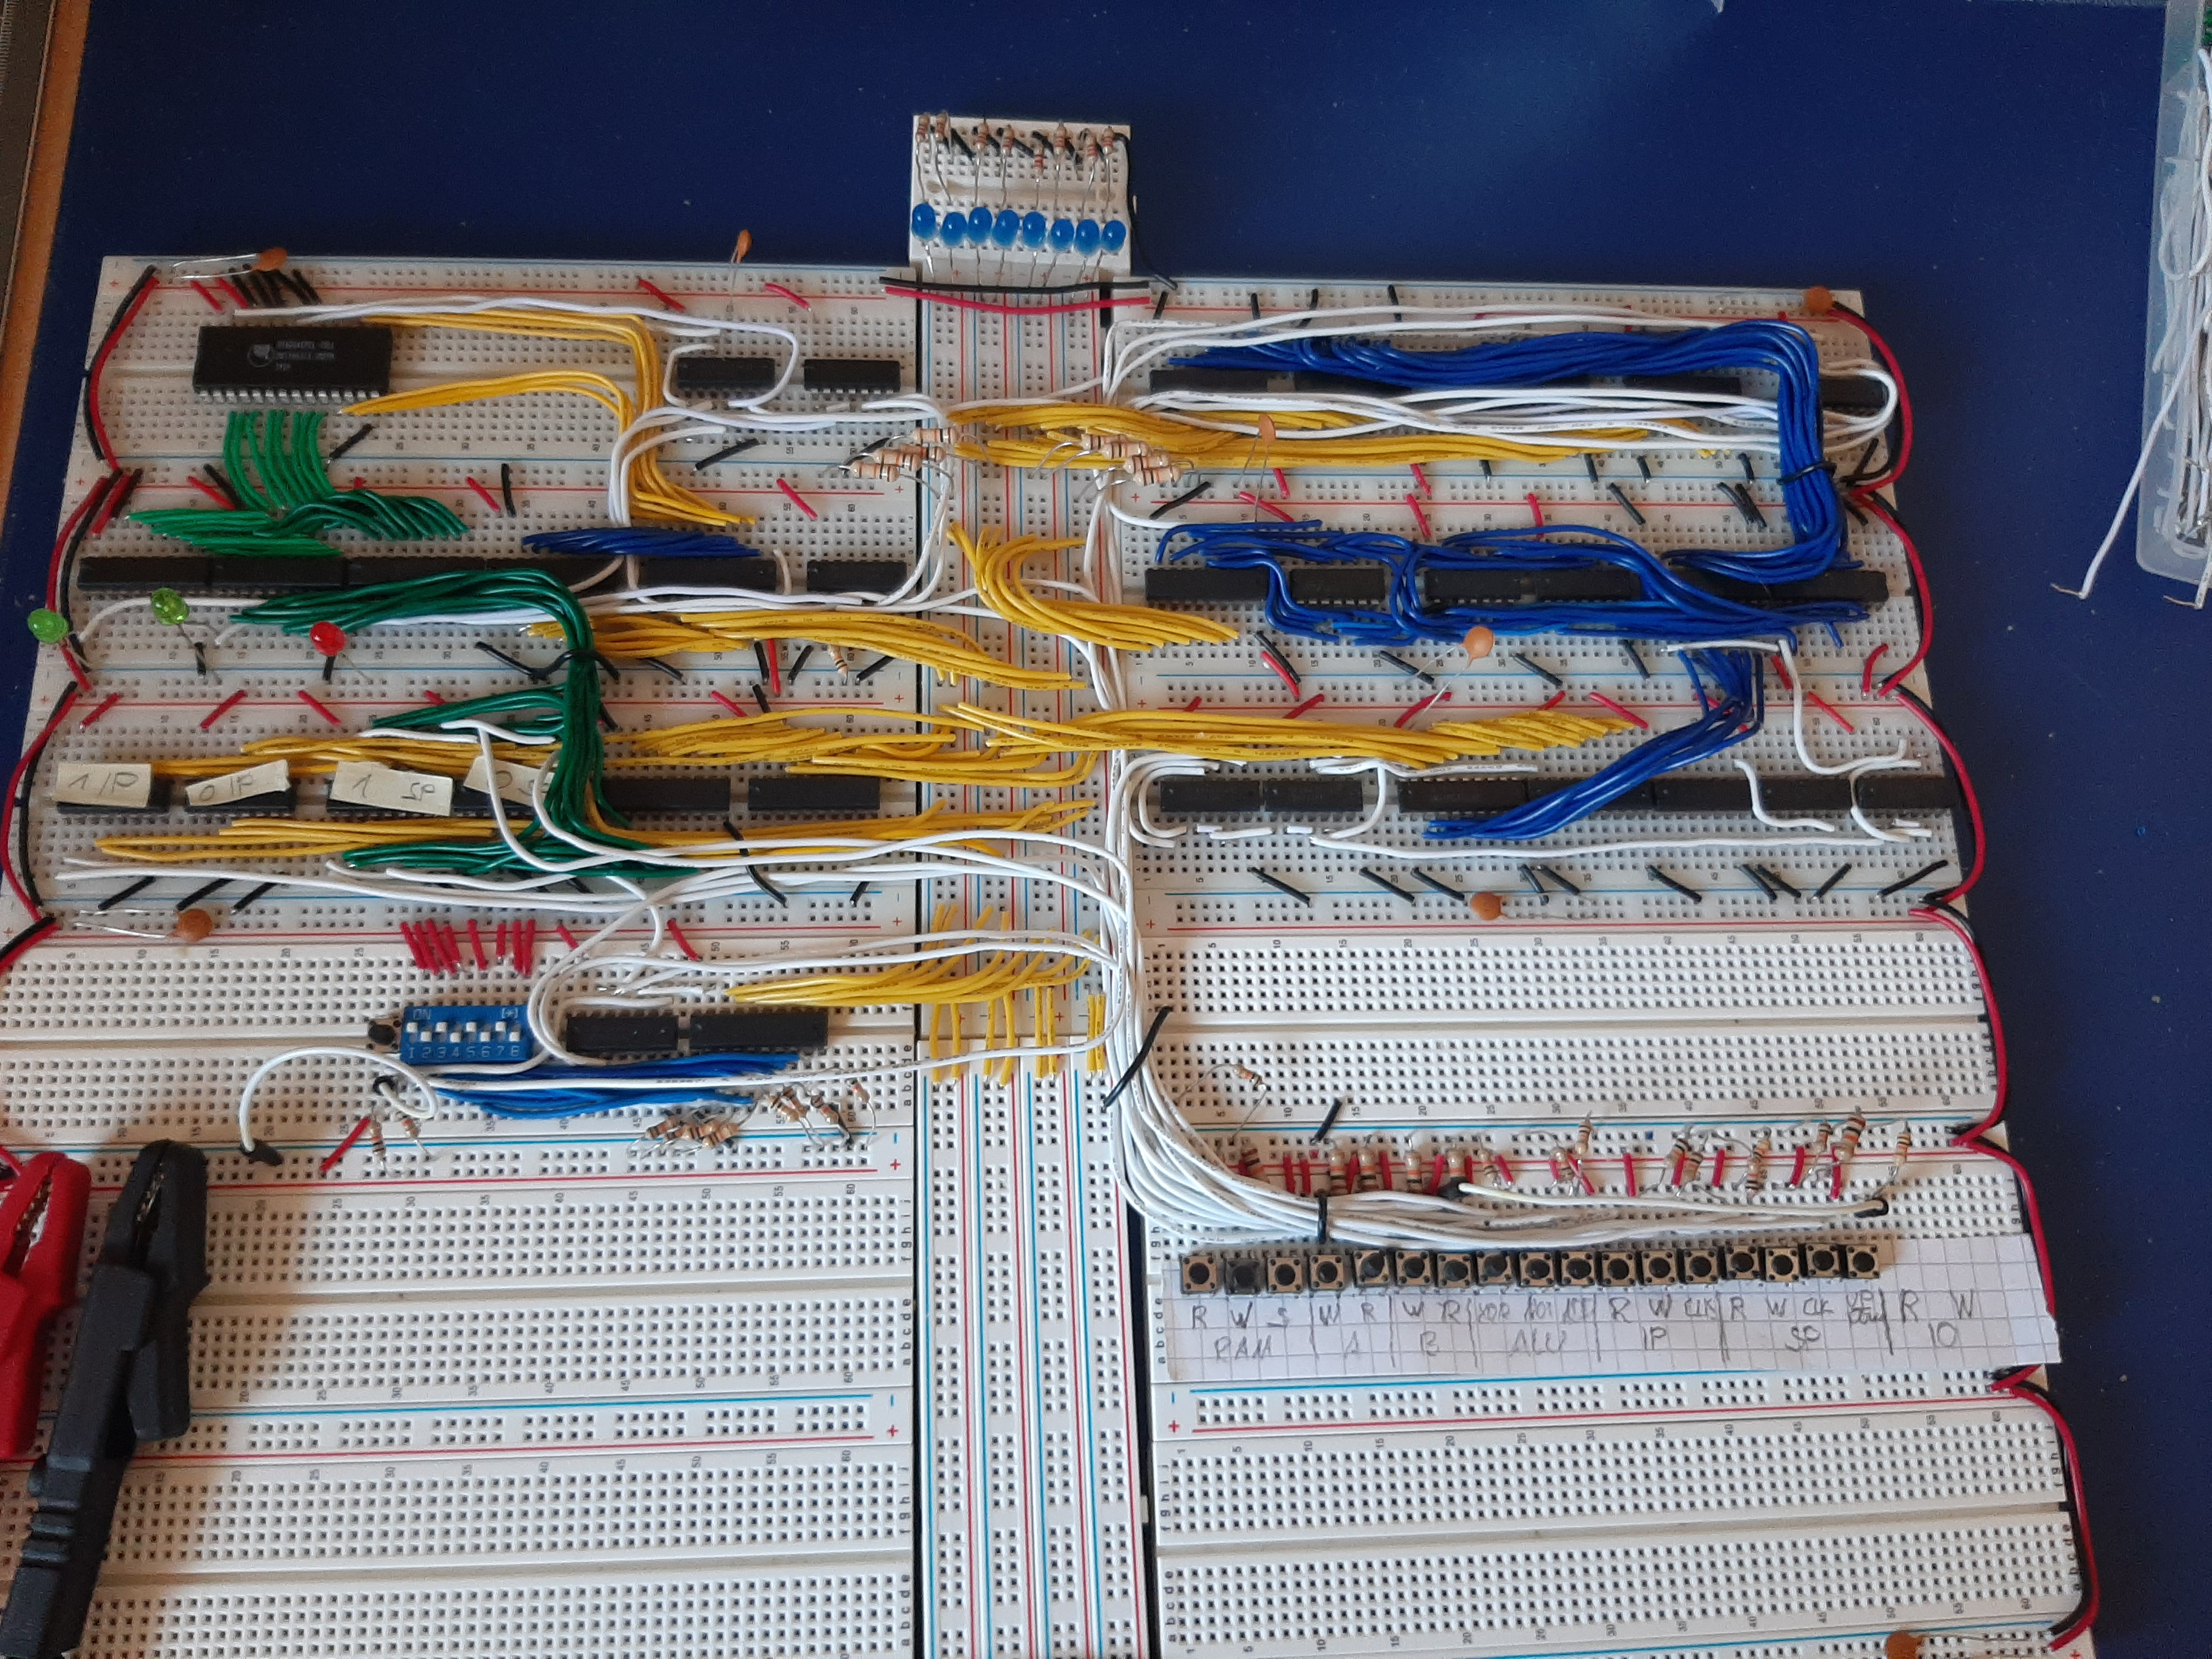
\includegraphics[width=0.5\textwidth]{Computer_V01_Overview_01}
        \end{center}
        \vspace{-20pt}
        \end{wrapfigure}
    Ein paar Monate später haben wir uns dann dazu entschieden, tatsächlich einen eigenen 8-bit-Computer zu bauen und haben auch bald angefangen erste Versuche auf dem Breadboard zu entwickeln.
    Es gab noch weder eine Möglichkeit diese erste Version automatisch zu betreiben, noch Daten zu schreiben/speichern, oder irgendwie mit der Umgebung zu interagieren, nur 3 Register, 2 Operationen und viele Knöpfe zum Bedienen.


    \section{Gebrauch von Platinen}
    \subsection{weshalb Platinen}

        \begin{wrapfigure}{r}{0.4\textwidth}
        \vspace{-40pt}
        \begin{center}
        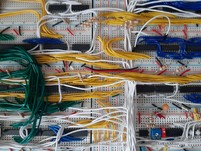
\includegraphics[width=0.37\textwidth]{Computer_V01_Chaos_07}
        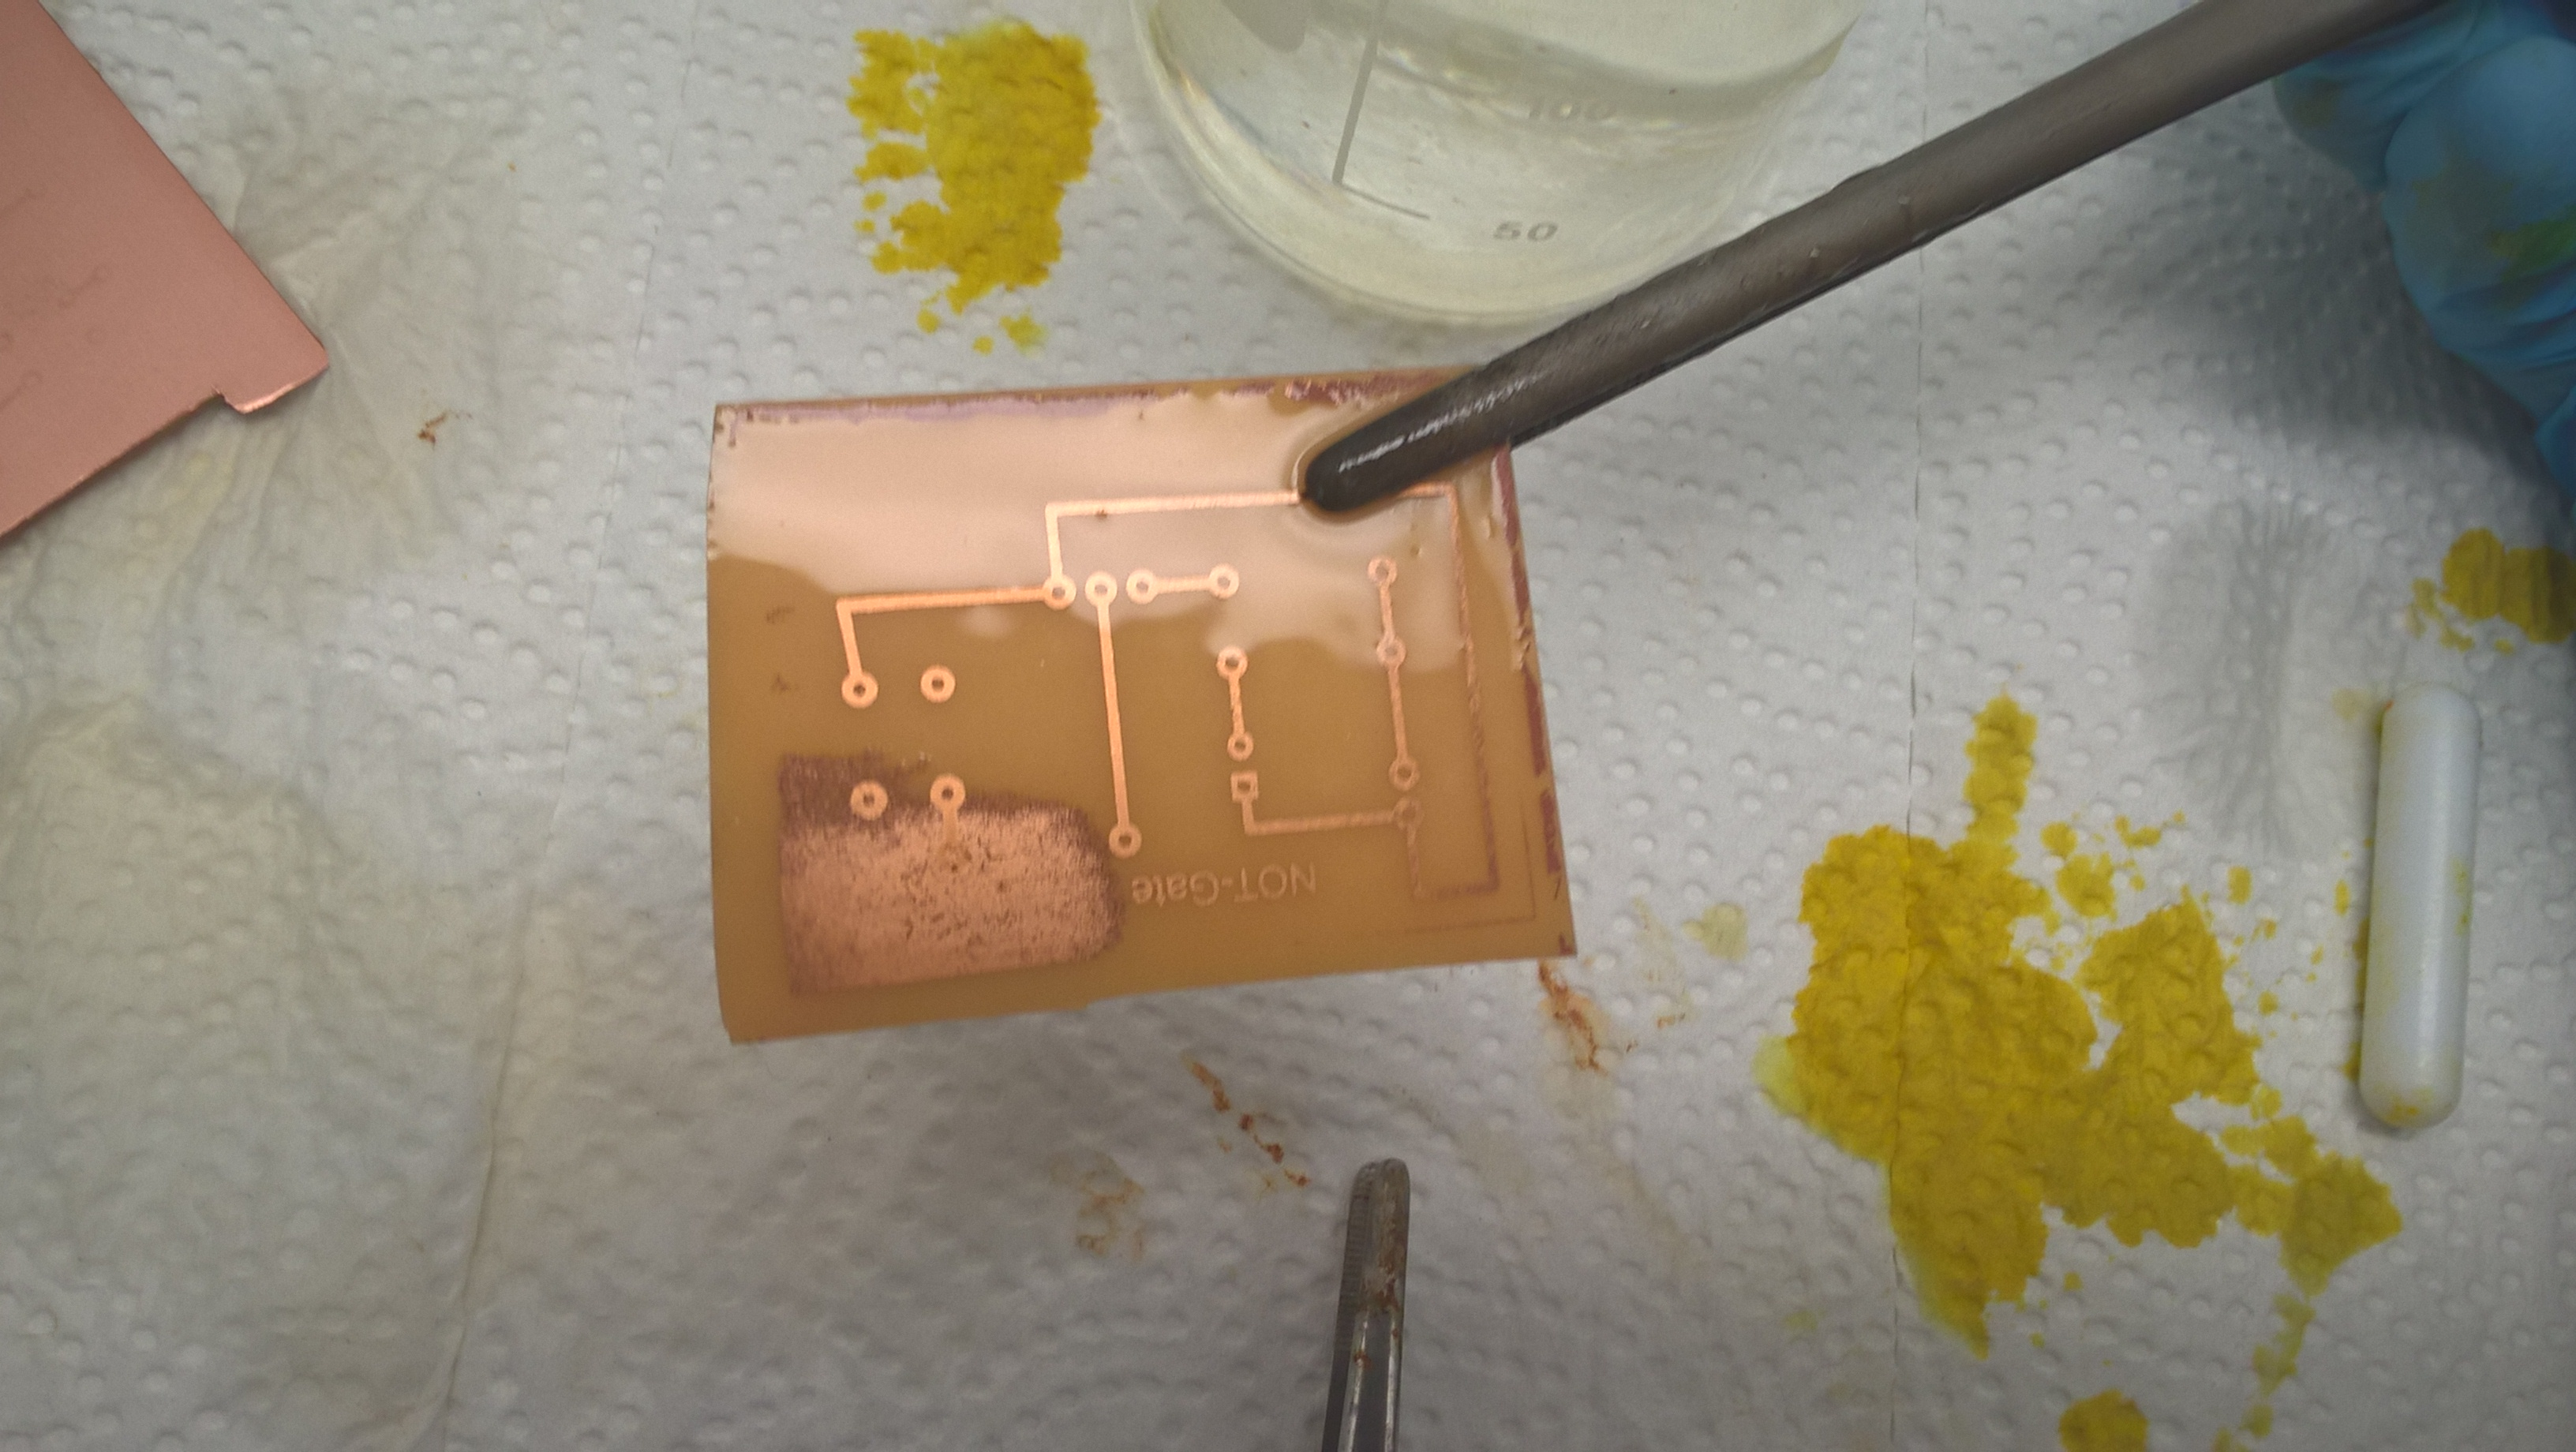
\includegraphics[width=0.37\textwidth,angle=0]{Handy/WP_20210704_20_54_21_Pro}
        \end{center}
        \vspace{-30pt}
        \end{wrapfigure}

    Bald war aber klar, dass ein einfaches Verwenden von flachen Kabel als Verbindung zwischen den Breadboards, das Kabelgewirr, dass wir bei dem Projekt von vor 2 Jahren gesehen haben
    und nach Möglichkeit vermeiden wollten, um ein übersichtlicheres Design zu erreichen, nicht lösen kann.

    Auf der Suche nach einer Alternative sind wir fast zwangsläufig auf Platinen gekommen, aber weil unser Computer ja nicht mehr wirklich selbst gemacht wäre, wenn wir diese nur professionell Ätzen lassen würden,
    wollten wir versuchen - zumindest einen Teil - selbst zu ätzen, auch wenn wir dadurch natürlich auf viele neue Probleme gestoßen sind...


    \newpage

    \subsection{Erste Versuche der Umsetzung}

        \begin{wrapfigure}{l}{0.4\textwidth}
        \vspace{-25pt}
        \begin{center}
        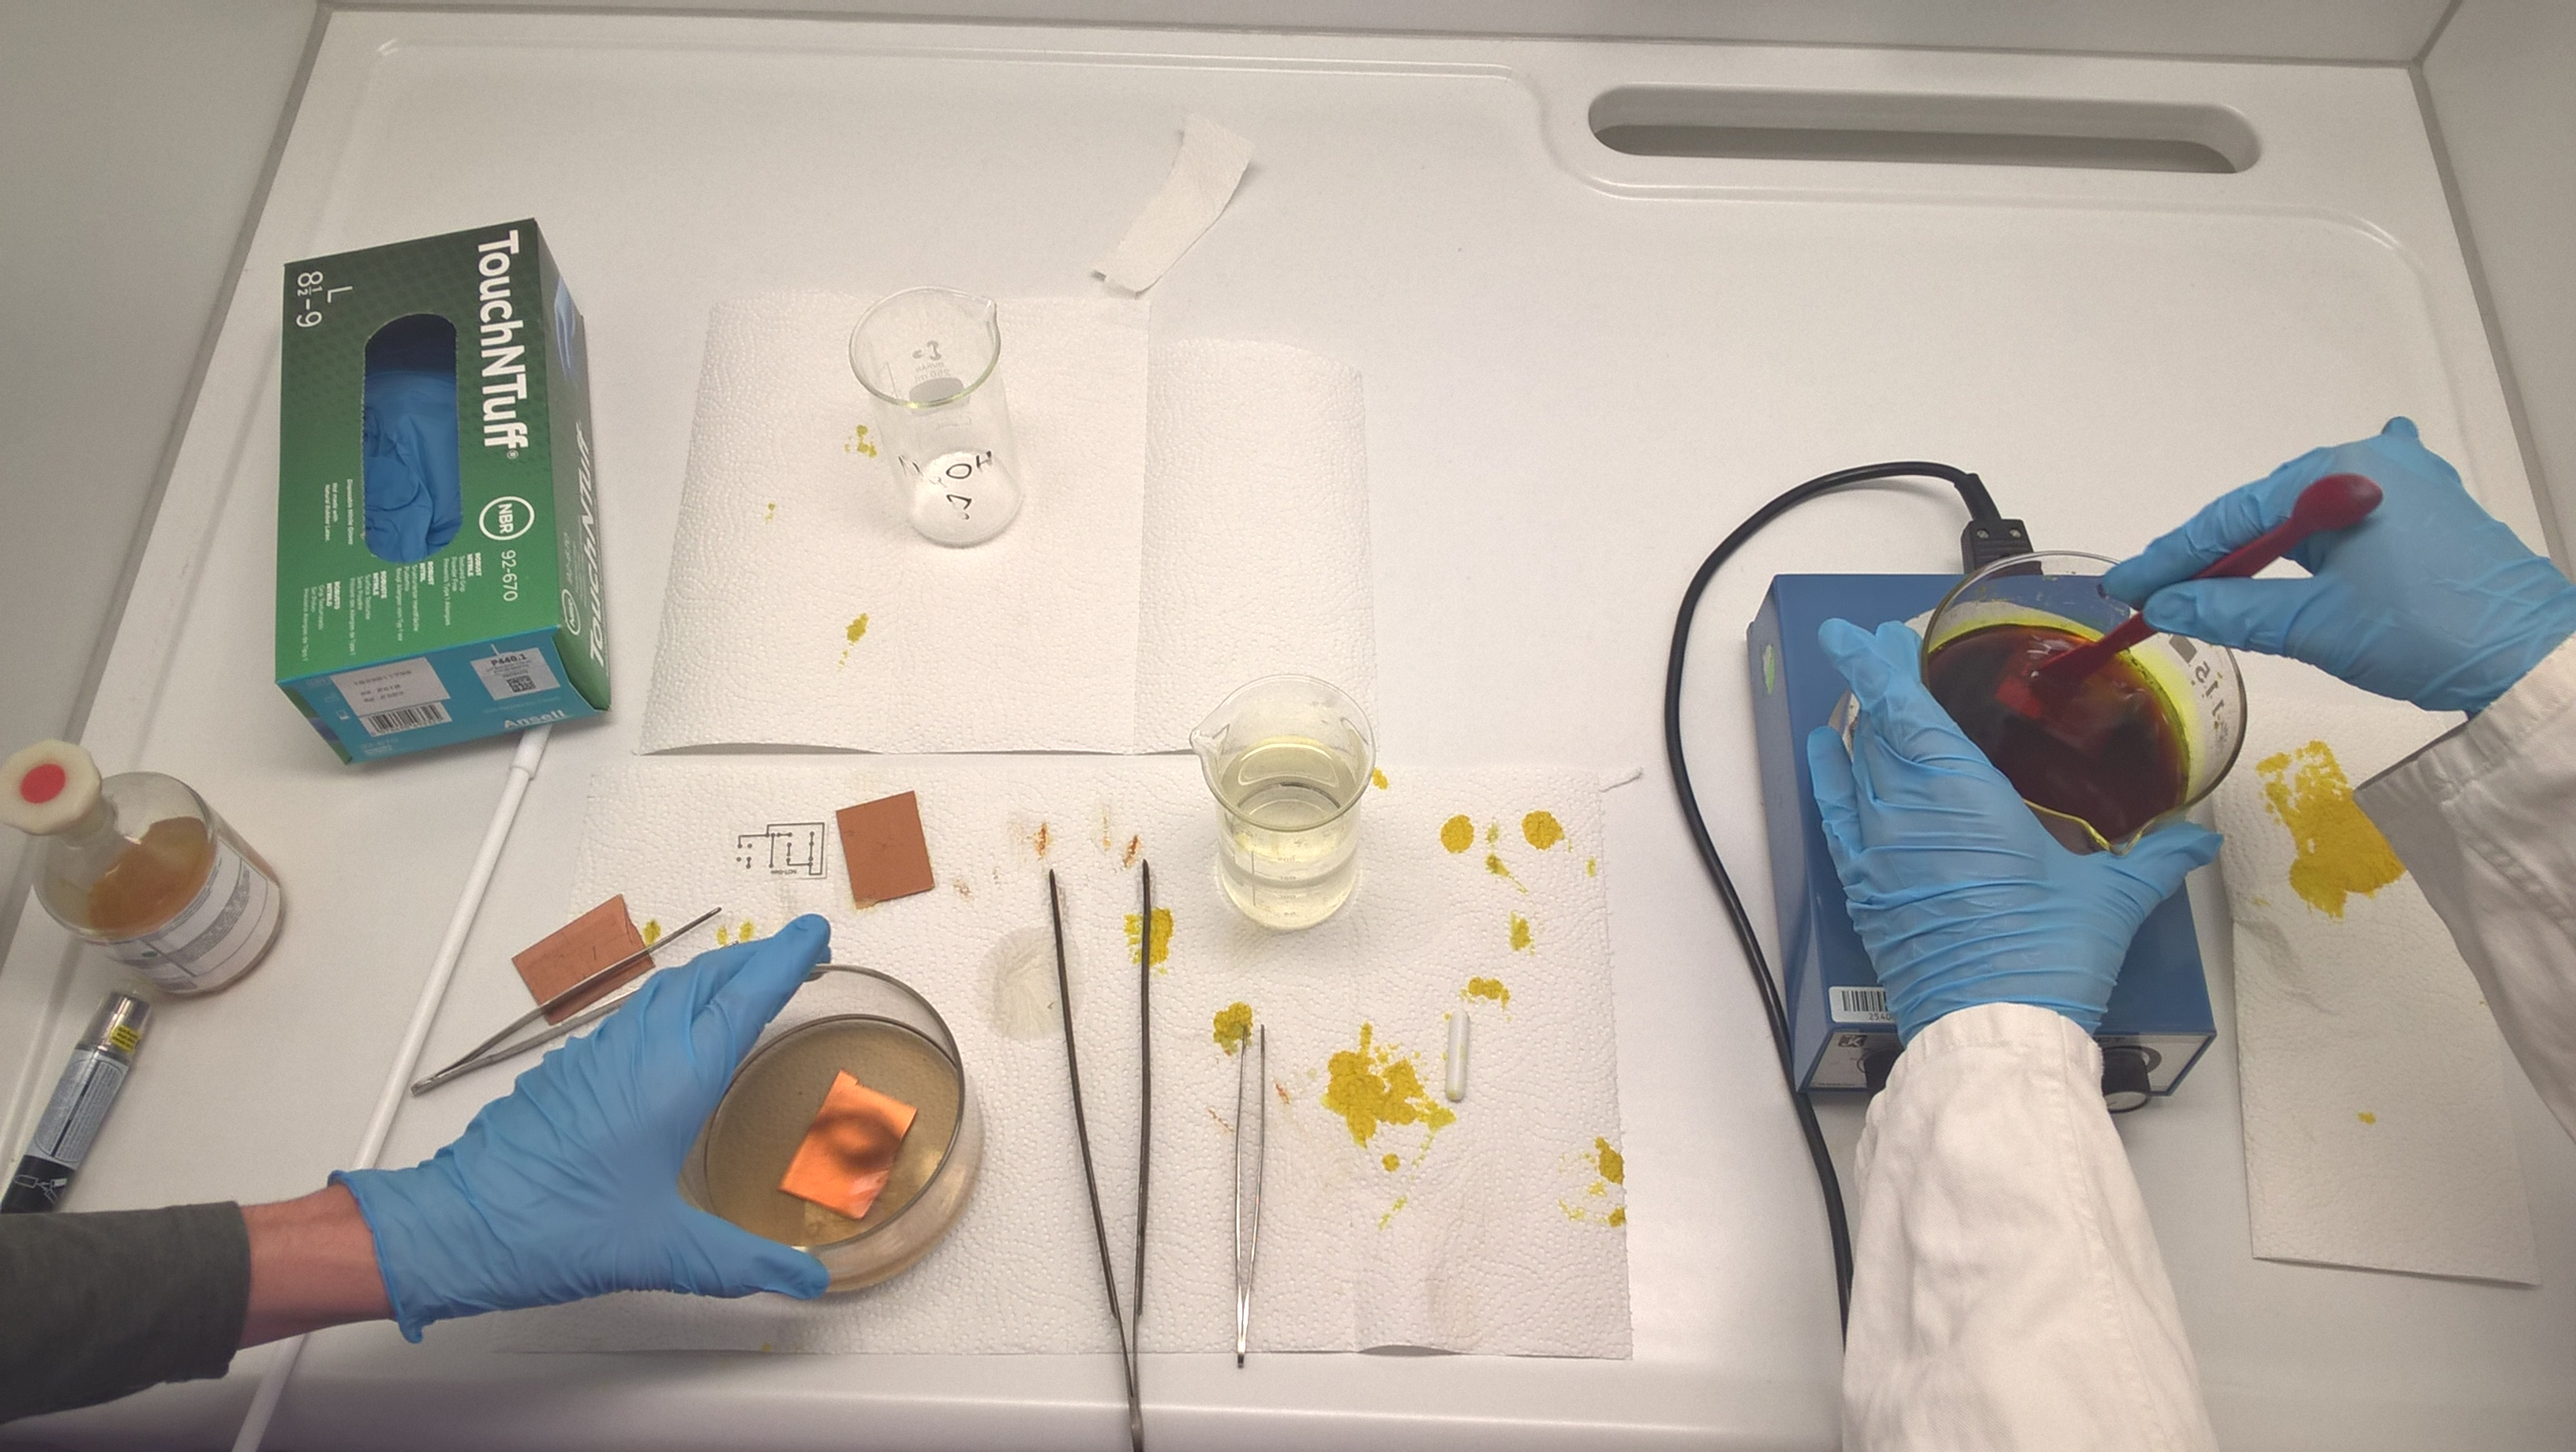
\includegraphics[width=0.4\textwidth,angle=0]{Handy/WP_20210704_20_40_03_Pro} %hier binn ich noch nicht ganz glücklich mit dem Bild
        \end{center}
        \vspace{-20pt}
        \end{wrapfigure}

    Was zu Beginn das Projekt vorangetrieben hat, hat ab diesem Punkt aber natürlich ein Problem dargestellt hat ist das Homeschooling, bei dem wir natürlich nicht Ätzen können.
    (wir hätten es natürlich zu Hause versuchen können, hatten da aber keine adequate Ausrüstung v.a. bzgl. Sicherheit)
    bis wir dann so weit waren erste Versuche zu machen war es dann schon Ende 2020.

    \subsection{Design}

        \begin{wrapfigure}{r}{0.65\textwidth}
        \vspace{-40pt}
        \begin{center}
        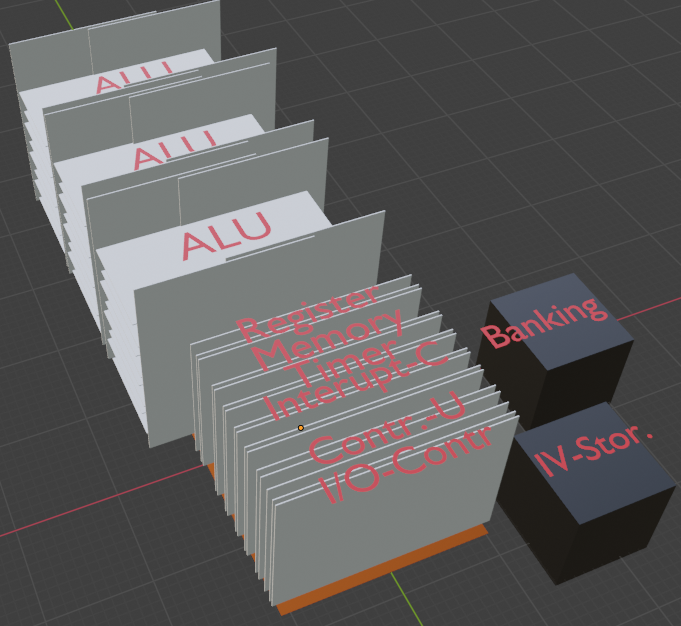
\includegraphics[width=0.55\textwidth]{3D_desighn_V21}
        \end{center}
        \vspace{-30pt}
        \end{wrapfigure}

    Nachdem es auch auf geätzten Platinen noch nicht automatisch ordentlich ist und eine derart große Platine für uns nicht machbar gewesen wäre, haben wir uns dann noch ein 3-Dimensionales Design ausgedacht.


    Offensichtlich ist das mit unseren aktuell geplanten Modulen: am Boden sitzt eine große Bus-Platine, auf der wir alle Module senkrecht aufstecken.
        \newline
        \newline
        \newline

    \newpage
    \section{Anforderungen V1}
    Im nächsten Lockdown hatten wir dann wieder viel Zeit zu planen, und der geplante Computer wurde immer komplexer.

    \subsection{Datenlänge}

    Aus den ursprünglich geplanten 8-bit wurden 16-bit Datenlänge:

        \vspace{-5pt}
        \fbox{%
        \parbox{1\textwidth}{

        Die Address- und Datenlänge besagt, wie viele Binäre Ziffern (bits) für eine Address und Daten verwendet werden.\\
        Je mehr Ziffern man verwendet desto größere Zahlen können in einer Operation verarbeitet werden wobei die maximal repräsentierbare Zahle $2^n - 1$ ist wenn $n$ die Anzahl der Binären Ziffern (= Bits) ist.\\
        \\
            $n$ teilbar durch $8$ zu machen, ist dabei relativ angenehm, weil $8$ bit = $1$ byte,\\
        und Bytes sind nun mal die grundlage für das meiste in der Informatik,\\
        zudem kommen einige elementar ICs, z.B. Buffer oder Register, immer mit 8 bits.\\
        \\
        Jedoch gilt je mehr Bits man verwendet, desto mehr Schaltung brauchen man, desto mehr Stromverbrauch, wodurch es für uns relativ schnell unrealistisch aufwendig wird\\
        \\
        Wir haben uns daher für $16$ bit entschieden, womit wir
            Zahlen bis zwischen $0$ und $65535$ darstellen können.\\
        Diese Menge ist gerade große genug, um für die meisten Programme große genüge Zahl abzubilden, aber trotzdem auf Platinen noch einigermaßen handhabbar.\\

        }%
        }
        \vspace{0pt}

    \newpage
    \subsection{Memory}
    Um auch Daten oder Programme verwenden zu können haben wir dann als erstes noch einen Größeren Speicher hinzu gefügt: Memory

        \vspace{-5pt}
        \fbox{%
        \parbox{1\textwidth}{
        Memory ist in 65536 (weil wir genau so viele Adressen in unseren 16bit speichen können) einzelne und unabhängige Speicherzellen (Jede 16 Bit große) aufgeteilt.\\
        Der Computer kann damit auf $65536 \text{ words}$ oder $131072 \text{ bytes}$ ($\approx 128 \text{ kib}$) direkt zugreifen.\\
        (Die Größe messen wir in words (w) oder in kilowords (kiw), wobei $1 \text{ word} = 2 \text{ bytes} = 16 \text{ Bit}$ sind.)\\
        \\
        Memory wird dabei über LD- und STR-Instruktionen gesteuert.\\
        Die LD-Instruktion kopiert einen Wert aus Memory und schreibt ihn in ein Ziel-Register, während STR an der angegebenen Adresse den Wert mit dem Wert des Quellen-Register überschreibt.\\

        }%
        }
        \vspace{0pt}

    Um aber noch mehr speicher zu bekommen und das später erwähnte Berechtigungssysten möglichst einfach um zu setzen haben wir noch Banken hinzu gefügt:

        \vspace{-5pt}
        \fbox{%
        \parbox{1\textwidth}{
        Banken sind externe Memory Module, die eingesteckt werden können.
        Alle Banken sind gleich groß ($16\text{kiw} = 32\text{ kib}$) und der Computer unterstützt maximal $65536$ unterschiedliche Banken.
        Jede Bank hat dabei eine ID (BID), die von $0$ bis $65535$ reicht.

        Der Computer hat zwei Bank-Slots (Slot 1 \texttt{0x8000 - 0xbfff} und Slot 2 \texttt{0xc000 - 0xffff}).
        \newline
        \newline
        Es kann auf jede dieser Slots eine der theoretisch $65536$ Banken legen, wobei

        Bank $1$ dafür gedacht ist, dass jedes normale Programm in seiner eigenen Bank dort eingefügt wird, sodass in den Programmen absolute Memory Adressen verwendet werden können, weil das Programm immer an der gleichen Stelle liegt.
        außerdem wird in der Bank auch der Stack des Programms gespeichert, sodass dieser von anderen Prozessen auch nicht durcheinander gebracht werden kann.

        und Bank $2$ als potentiellen zusätzlichen Speicher des Programms, oder als allgemeineren Speicherort, um zwischen den Programmen daten zu übermitteln.

        }%
        }


    \subsection{Logik-Operationen und konditionale jumps}
    Um die neuen Möglichkeiten durch 16-bit auch sinnvoll nutzen zu können haben wir dann noch eine ganze Reihe an neuen Operationen hinzugefügt:
    Viele Logikoperationen bis hin zur Hardware- Multiplikation und komplexere konditionale Jumps.
    \begin{center}
        \begin{table*}
            \caption{\label{table:instructions}Instruktions-Satz}
            \begin{tabular}{l | l l l l | l}
                Ins-ID & Name & op1 & op2 & op3 & Beschreibung \\
                \hline
                \texttt{0x00} & NOP  &  &  &  & Kein Effekt  \\
                \hline
                \texttt{0x01} & MOV  & reg &  & reg/c & op1 $=$ op3\\
                \texttt{0x02} & ADD  & reg & reg & reg/c & op1 $=$ op2 $+$ op3 \\
                \texttt{0x03} & SUB  & reg & reg & reg/c & op1 $=$ op2 $-$ op3 \\
                \texttt{0x04} & MUL? & reg & reg & reg/c & op1 $=$ op2 $*$ op3 \\
                \texttt{0x05} & MULOF& reg & reg & reg/c & op1 $=$ Overflow op2 $*$ op3 \\
                \texttt{0x05} & DIV? & reg & reg & reg/c & op1 $=$ op2 $/$ op3 \\
                \texttt{0x06} & XOR  & reg & reg & reg/c & op1 $=$ op2 $\oplus$ op3 \\
                \texttt{0x07} & AND  & reg & reg & reg/c & op1 $=$ op2 $\land$ op3 \\
                \texttt{0x08} & OR   & reg & reg & reg/c & op1 $=$ op2 $\lor$ op3 \\
                \texttt{0x09} & NOT  & reg &  & reg/c & op1 $=$ $\lnot$op3 \\
                \hline
                \texttt{0x0a} & STR  & reg & reg & reg/c & memory[op2 + op3] = op1  \\
                \texttt{0x0b} & LD   & reg & reg & reg/c & op1 = memory[op2 + op3] \\
                \texttt{0x0c} & BNK1 &  &  & reg/c & Setzt BID für Bank-Slot1 \\
                \texttt{0x0d} & BNK2 &  &  & reg/c & Setzt BID für Bank-Slot2 \\
                \hline
                \texttt{0x0e} & PUSH &  &  & reg/c & SP--; memory[SP] = op1 \\
                \texttt{0x0f} & POP  &  &  & reg & op3 = memory[SP]; SP++ \\
                \texttt{0x10} & CALL &  &  & reg/c & \vtop{
                    \hbox{\strut memory[SP] = IP; SP++;}
                    \hbox{\strut IP = op3}} \\
                \texttt{0x11} & RET  &  &  &  & IP = memory[SP]; SP++ \\
                \hline
                \texttt{0x12} & TEST & reg &  & reg/c & Vergleicht op1 und op3 \\
                \texttt{0x13} & ME   & reg &  & reg/c & op1 = op3 if E \\
                \texttt{0x14} & MG   & reg &  & reg/c & op1 = op3 if G \\
                \texttt{0x15} & ML   & reg &  & reg/c & op1 = op3 if L \\
                \texttt{0x16} & MS & reg &  & reg/c & op1 = op3 if SUP \\
                \texttt{0x17} & MI & reg &  & reg/c & op1 = op3 if OINT \\
                \texttt{0x18} & MOFadd  & reg &  & reg/c & op1 = op3 if O \\
                \texttt{0x19} & MOFsub  & reg &  & reg/c & op1 = op3 if O \\
                \hline
                \texttt{0x1a} & IOUT & reg &  & reg/c & IIO[op1] = op3/c \\
                \texttt{0x1b} & DOUT & reg &  & reg/c & DIO[op1] = op3/c \\
                \texttt{0x1c} & DIN  & reg &  & reg & op3 = DIO[op1] \\
                \texttt{0x1d} & AIO  & reg &  &  & Aktiviert IO[op1] \\
                \texttt{0x1e} & DIO  & reg &  &  & Deaktivieren IO[op1] \\
                \hline
                \texttt{0x1f} & INT  & & & & Löst einen Interrupt aus \\
                \texttt{0x20} & TM1  & & & reg/c & Modi Timer1 = op3 \\
                \texttt{0x21} & TM2  & & & reg/c & Modi Timer2 = op3 \\
                \texttt{0x22} & SSTL1 & & & reg/c & lower Stop Timer1 = op3 \\
                \texttt{0x23} & SSTL2 & & & reg/c & lower Stop Timer2 = op3 \\
                \texttt{0x24} & SSTH1 & & & reg/c & higher Stop Timer1 = op3 \\
                \texttt{0x25} & SSTH2 & & & reg/c & higher Stop Timer2 = op3 \\
                \texttt{0x26} & CFL  & reg & & & op1 = lower Clock Freq \\
                \texttt{0x27} & CFH  & reg & & & op1 = higher Clock Freq \\
                \hline
            \end{tabular}
        \end{table*}
    \end{center}

    \subsection{IO-Ports}
    Dazu hat sich dann die Idee von einer komplexeren Umsetzung von Interaktion mit dem Computer eingeschlichen:
    universelle Ports zum Anschließen von (modifizierten) Festplatten, Sensoren, einfachen Tastaturen, LCD-Displays und der Vorstellung einer Grafikkarte, die echte Bildschirme betreiben kann.

        \vspace{-5pt}
        \fbox{%
        \parbox{1\textwidth}{
        die theoretisch 64ki Anschlüsse, die alle über eine Anschluss-ID angesprochen werden können, kommunizieren mit dem IO-Gerät über 4 Kommandos,
            die als 4 separate verbindungen zwischen dem Controller und dem Gerät umgesetzt sind:

        1. Einen Befehl an das IO-Gerät schicken (auf Programm-Ebene);

        2. Daten zu einem vorherigen Befahl an das Gerät schreiben;

        3. Die Anfrage der IO-Gerätes Daten an den computer zurück zu schreiben, was bei diesem normalerweise einen Interrupt auslöst

        4. Bestätigen des Computers, das das Externe Gerät schreiben darf.

        }%
        }

    \subsection{Berechtigungssysten}
    Die vermutlich die größte Änderung war danach, dass wir ein Berechtigungssystem einführen wollten.
    Dafür haben wir dann Flaggen, Interrupts und noch mehr Instruktionen hinzugefügt.
    \subsection{ROM}
    Um den Computer komplett unabhängig funktionsfähig machen zu können, haben wir uns dann überlegt einen Teil des RAMs durch ROM zu ersetzen, um automatisch Programme von einem externen Speichermedium laden zu können.
    \subsection{Banking}
    Nachdem uns $2^{16}$= 65536 Speicherzellen (jede einen 16-bit Wert beinhaltend) also 128kiB Daten in Memory bei so vielen Anforderungen dann doch etwas wenig erschienen
    und wir die Idee von mehreren Prozessen, die abwechselnd ausgeführt werden, verlockend war haben wir uns dann entschieden durch eine neue Instruktion, mit der wir Teile des Arbeitsspeichers auswechseln können (Banking),
    beides zu ermöglichen. [Link zu Dokumentation v0.2]


    \subsection{Nützung eines 2. Busses}

    Um Memory innerhalb einer Instruktion zu beschreiben, muss dieses sowohl eine 16-bit Adresse über die Position in Memory erhalten,
    als auch den 16-bit Wert, der dort gespeichert werden soll,
    damit diese beiden Daten parallel übermittelt werden können brauchen wir also 2*16bit.
    Wir hätten dafür natürlich auch irgendwelche Kabel verlegen können, aber wir wollen in unserem System die Daten immer auf dem Bus haben, damit diese auch von anderen Modulen gelesen werden könnten, und die Adresse muss im Anwendungsfall als Stack vor benützung um eins erhöht oder veringert werden, was in unserem System durch die ALU erfolgen sollte, wobei diese nur auf den Bus ihre Daten ausgaben kann.

    \section{Tests}
    \subsection{Breadboard test}
        \begin{wrapfigure}{r}{0.65\textwidth}
        \vspace{-40pt}
        \begin{center}
        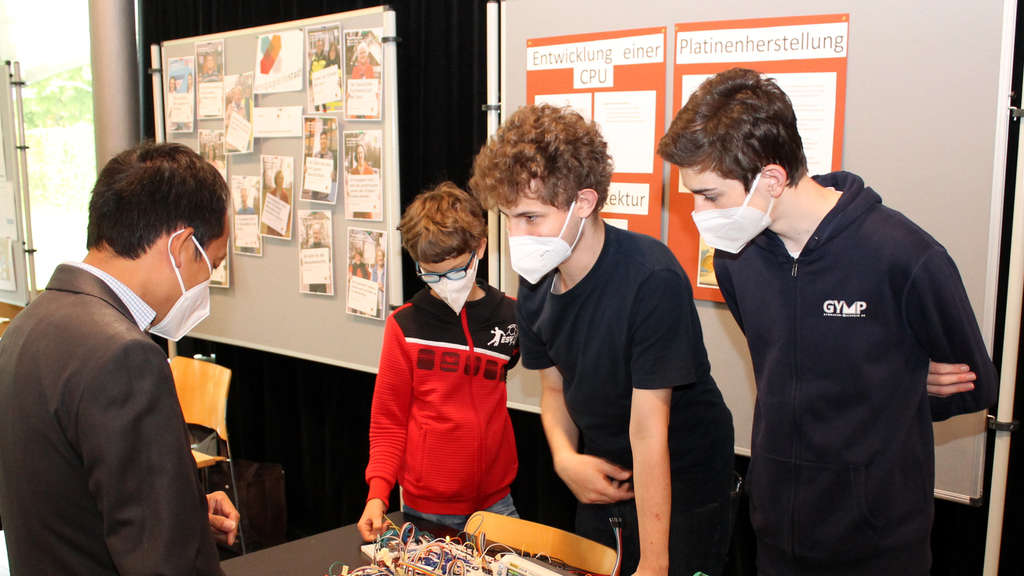
\includegraphics[width=0.55\textwidth]{Perspektive_P}
        \end{center}
        \vspace{-50pt}
        \end{wrapfigure}
    Zwischendurch haben wir dann für die Einladung zu der lokalen Veranstaltung
    $"$Persvektive P$"$ am 15.07.2021 wieder einen Prototyp auf dem Breadboard gebaut, wobei auch diese Version sehr unvollständig war.

    \subsection{Geschwindigkeit}
        \begin{wrapfigure}{r}{0.4\textwidth}
        \vspace{-20pt}
        \begin{center}
        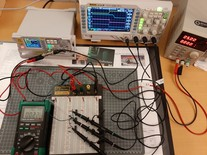
\includegraphics[width=0.4\textwidth]{20211208_200750_}
        \end{center}
        \vspace{-20pt}
        \end{wrapfigure}

    Um einen eindruck zu bekommen, wie komplex unsere programme werden können, ohne übermäßig lange zu brauchen, haben wir dann versucht zu errechnen, wie schnell wir den Computer maximal laufen lassen können, ohne fehlerhafte Ergebnisse zu erhalten.
    Also haben den "Propagation-delay", die Zeit, bis der Chip den Output liefert, den der laut der Eingabe haben müsste, aller Komponenten gemessen, die wir verwenden wollen.
    die meisten Chips, die wir jetzt vorhaben zu verwenden haben eine Verzögerung von ungefähr 8 Nanosekunden, allerdings haben wir bei den verschiedenen versionen, die wir getestet haben, teilweise weitaus höhere Werte bis zu 150ns erreicht, was an sich noch nicht so schlecht ist, aber wenn wir damit rechnen, dass wir reihen von bis zu 40 Chips in einem Clock-Zyklus haben, limitiert das die Geschwindigkeit schon sehr.

    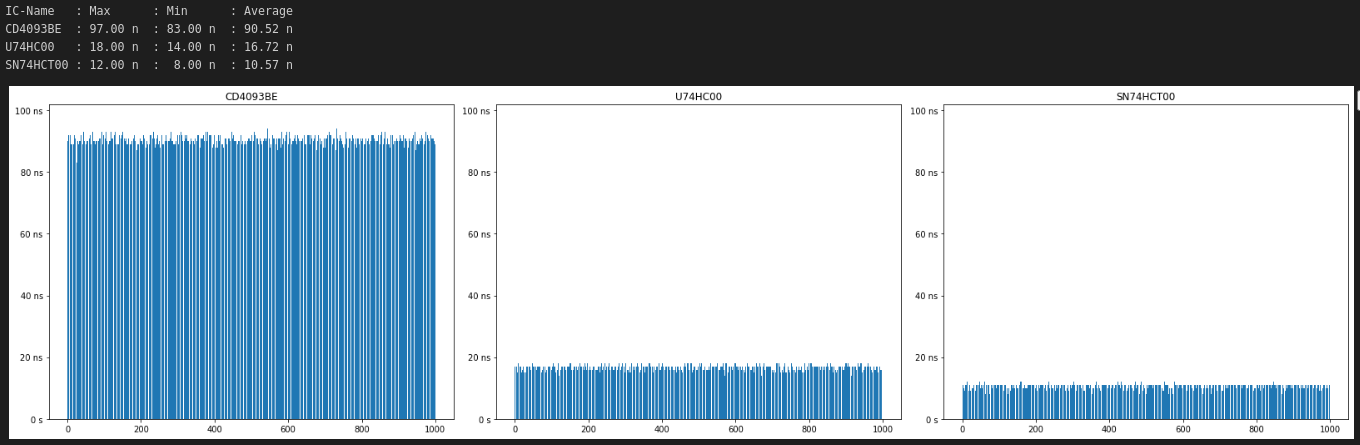
\includegraphics[width=\textwidth]{NANDs_Result_Rising}


    \subsection{Funktionsweise Chips}
    Wir wollen als basis für unseren Computer ja Chips kaufen, aber wie funktionieren die eigentlich?
    Wir haben also versucht den Aufbau herauszufinden, indem wir einfach einen geöffnet haben, wobei $"$Einfach$"$ nicht so ganz stimmt, weil die Hülle aus Epoxidharz besteht, was sich fast nicht auflösen lässt.
    Also mussten wir mechanisch abtragen, also Schleifen.

    Leider haben wir es damit nie geschafft das gesamte Silizium/die Verbindungsbahnen frei zu legen, sodass wir keinen schaltplan erstellen könnten,
    es gab uns aber trotzdem eine beeindruckende persönliche Einsicht:


        \begin{figure}[h]
        \begin{subfigure}[b]{0.3\textwidth}
            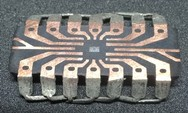
\includegraphics[width=\textwidth]{WP1_09}
            \end{subfigure}
        ~
        \begin{subfigure}[b]{0.3\textwidth}
            \includegraphics[width=\textwidth]{WP_20211029_143251_}
            \end{subfigure}
        ~
        \begin{subfigure}[b]{0.3\textwidth}
            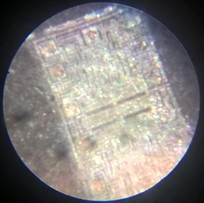
\includegraphics[width=\textwidth]{WP_20210917_16_56_15}
            \end{subfigure}
        \end{figure}


    \section{Umsetzung}
    \subsection{Programmierung}

        \begin{wrapfigure}{r}{0.6\textwidth}
        \vspace{-30pt}
        \begin{center}
        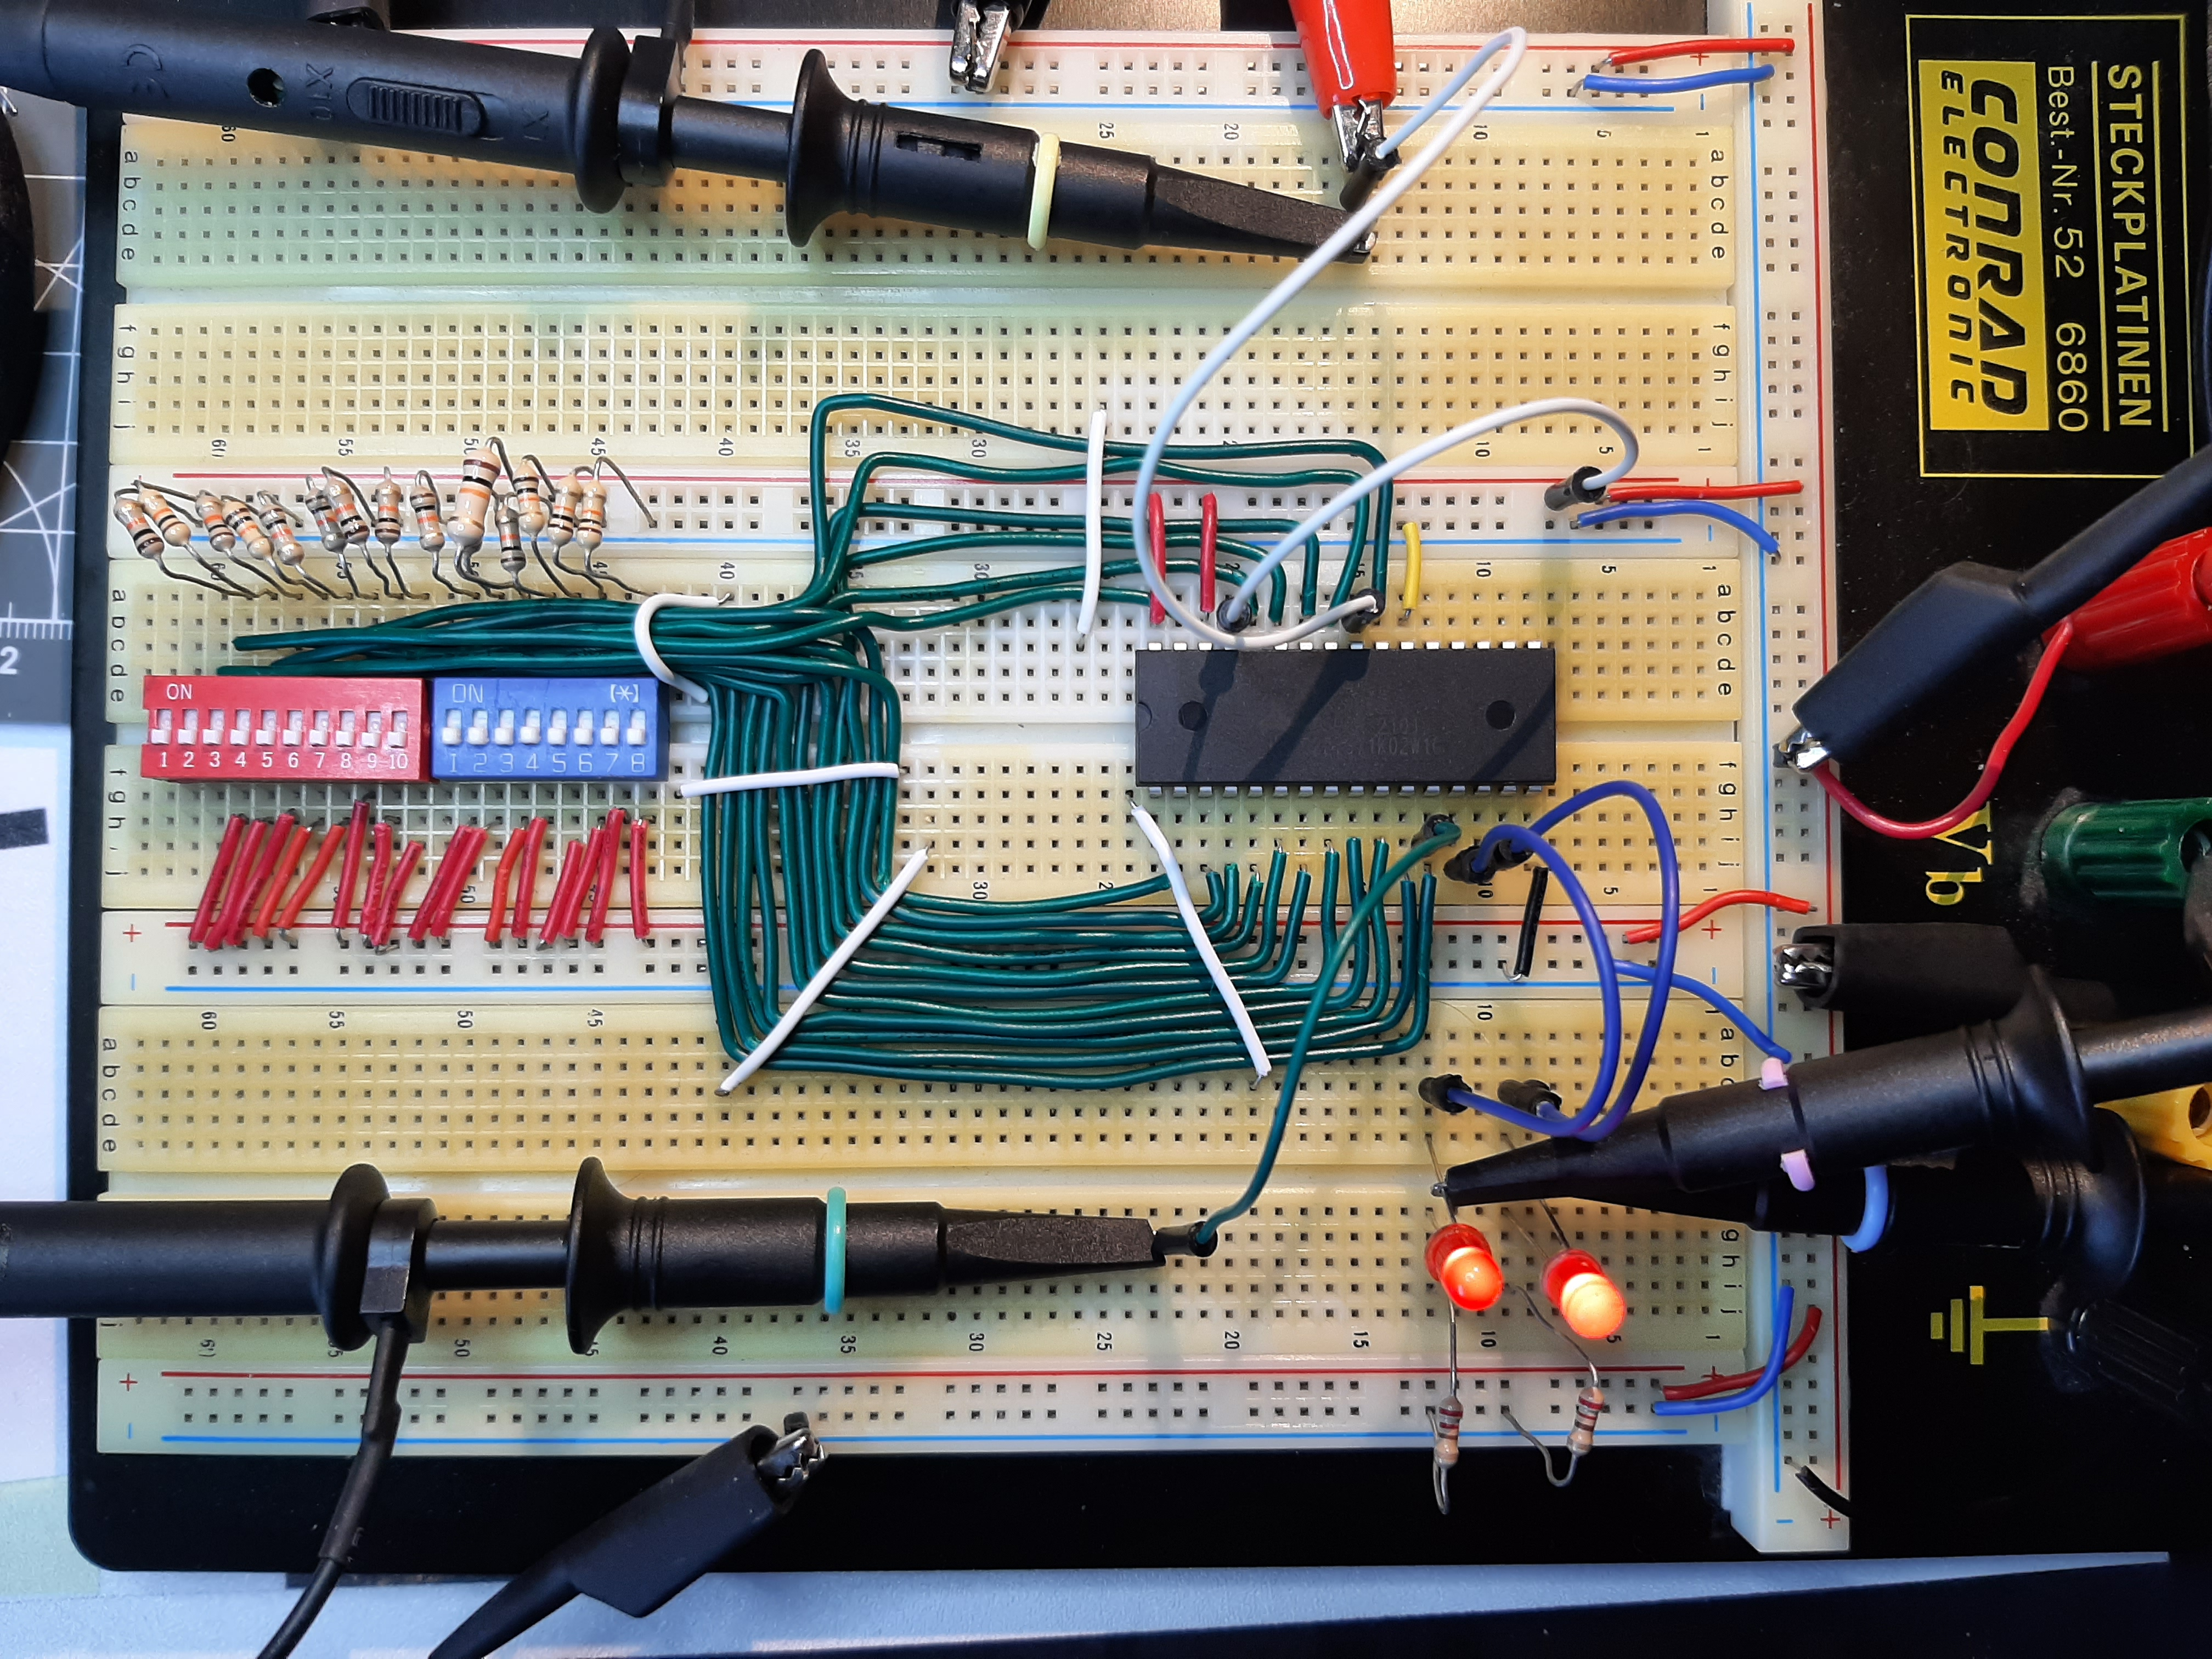
\includegraphics[width=0.6\textwidth]{ROM_Programmer_Manual_01}
        \end{center}
        \vspace{-20pt}
        \end{wrapfigure}

    Um den ROM-Chip zu programmieren haben wir zwar mal kurz ein bisschen manuell über Schalter programmiert, aber nachdem das offensichtlich zu lange brauchen würde haben wir dann einen Arduino (um genau zu sein, einen ESP32) programmiert und an die pins des ROM-Ch8ips angeschlossen.
    Der Arduino bekommt die zu schreibenden bits wiederum aus einem Python-Programm, das den Assembler in Maschinensprache (eine binary Datei) umwandelt.

    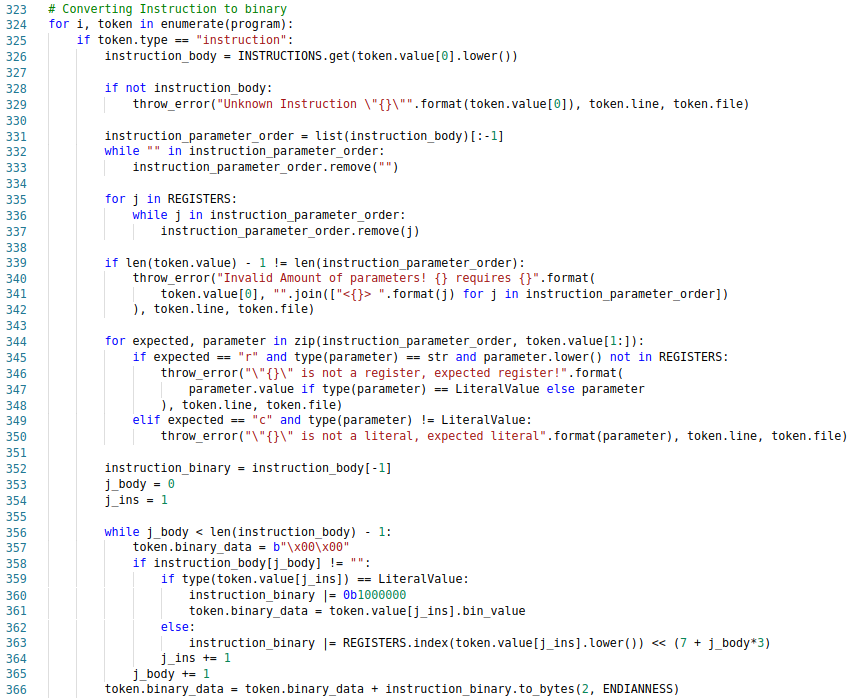
\includegraphics[width=0.8\textwidth]{assembler_code}

    \subsection{weitere tests zum Ätzen}
        \begin{wrapfigure}{r}{0.6\textwidth}
        \vspace{-40pt}
        \begin{center}
        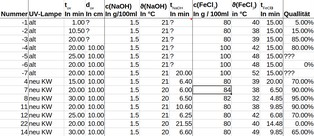
\includegraphics[width=0.6\textwidth]{aetzen_tabelle}
        \end{center}
        \vspace{-20pt}
        \end{wrapfigure}
    Im Schuljahr 2021-2022 haben wir dann wieder weitere Tests zum Ätzen - dieses mahl sowohl erfolgreicher, als auch besser Dokumentiert, um die optimalen Belichtungs- und Ätzzeiten zu finden.

    \subsection{Spezifikation}
    Gleichzeitig haben wir auch angefangen unsere erste vollständige Version der Spezifikation zu schreiben siehe: https://www.mediafire.com/file/9iz9wlpiuwhr1ln/HandBuch.pdf/file

    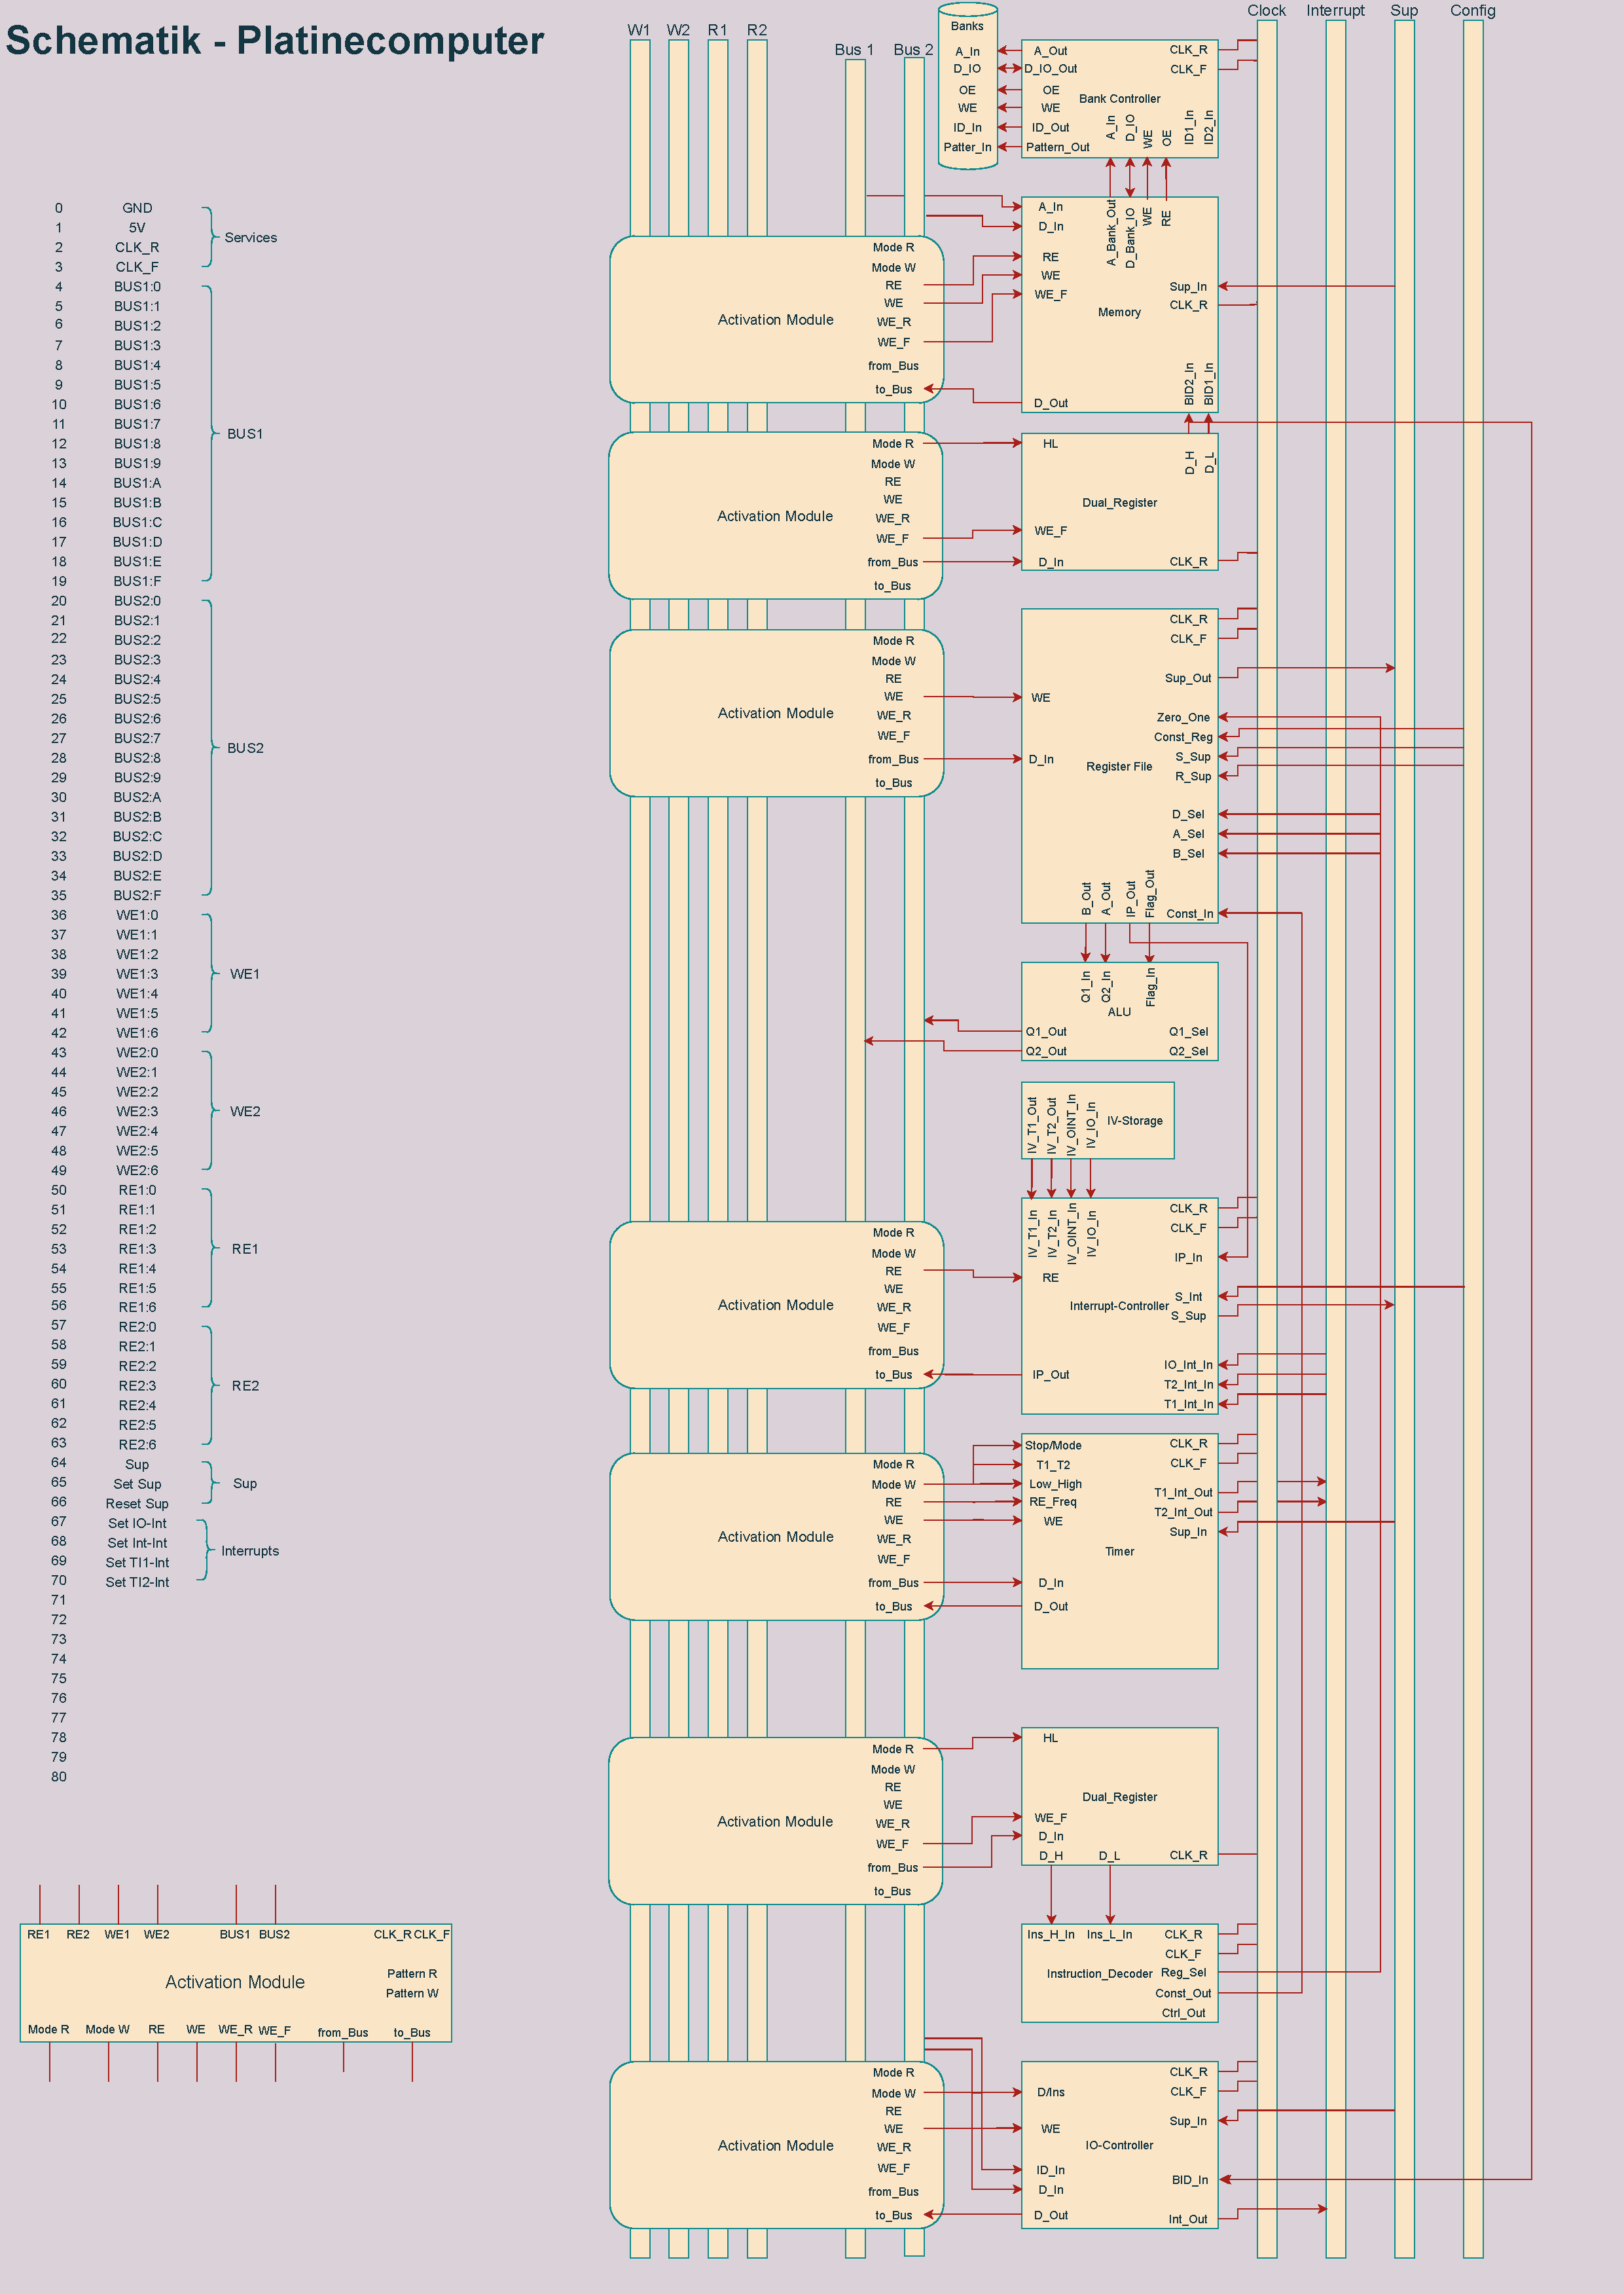
\includegraphics[width=0.612\textwidth, ]{arch.drawio}
    
    \subsection{Desighnen der Schaltungen}

        \begin{wrapfigure}{r}{0.7\textwidth}
        \vspace{-40pt}
        \begin{center}
        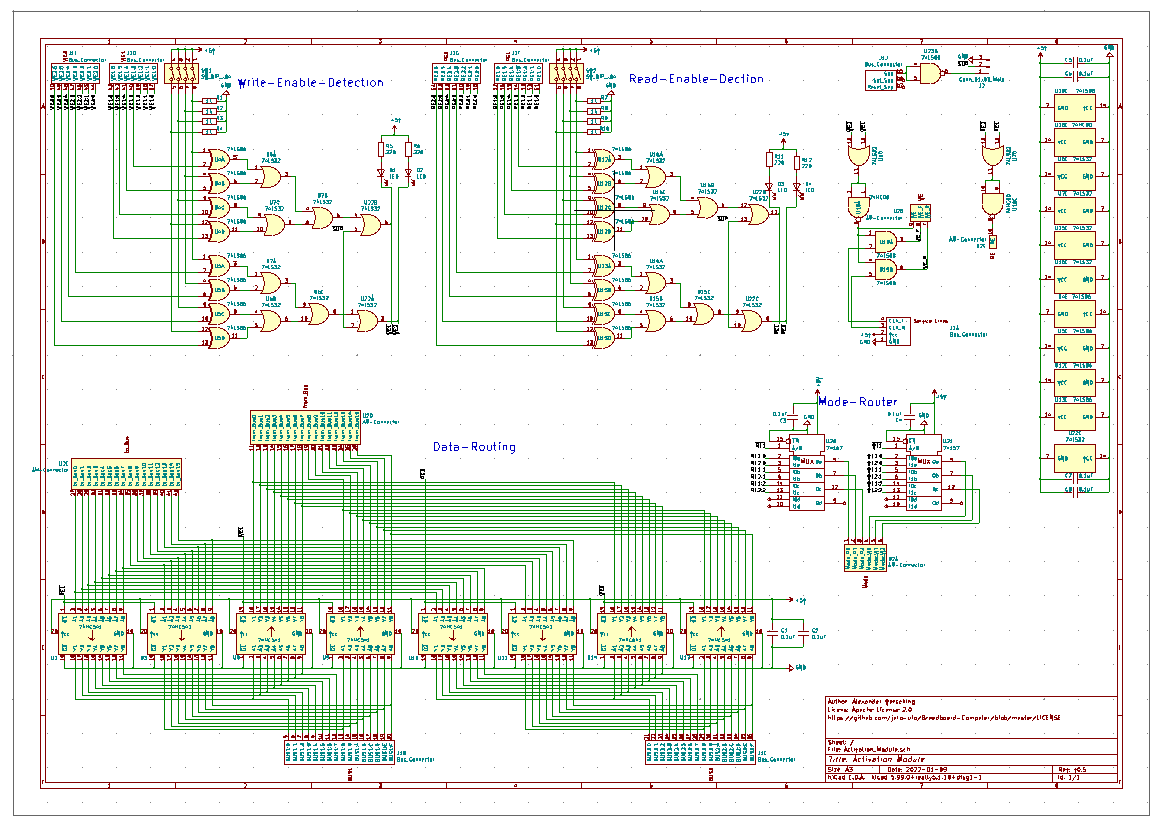
\includegraphics[width=0.65\textwidth]{kicad_schematic}
        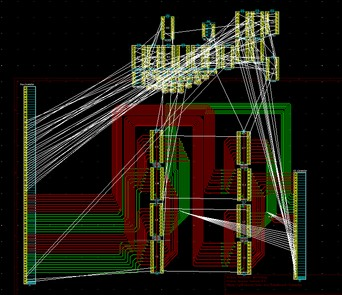
\includegraphics[width=0.65\textwidth]{kicad_pcb}
        \end{center}
        \vspace{-20pt}
        \end{wrapfigure}
    Zum designen haben wir uns schlussendlich darauf festgelegt, dass wir die Schaltungen zuerst in dem Logiksimulationsprogramm Logisim erstellen,
    und danach den Plan noch einmal als Ätzbaren Schaltplan erstellen, wobei wir hierfür kein wirklich zufriedenstellendes Produkt finden konnten.
    Schließlich haben wir uns vor allem wegen der einfachheit es zu bekommen und Installieren für KiCad entschieden, was uns allerdings ziemlich viel frust beschert hat.


\end{document}